\par To design a controller that is robust against approximation errors, we quantify the errors introduced due to coarse-grained approximations as well as variable lossy compression and use it to design an approximation-aware controller.
Initially, we need to identify the system state parameter(s) affected by the approximations. 
For \gls{lkas}, the lateral deviation $\yL$ is affected by approximation. 
We quantify the error ($e_i$) due to approximation for the setting S$i$ as the covariance of the calculated $y_L^{i}$ for the approximation setting S$i$ with respect to the calculated $y_L^{0}$ for the accurate setting S0, i.e.,  
\begin{math}
e_i=\frac{1}{n}\sum_{j=1}^{n}(y_{L_j}^{i}-y_{L_j}^{0})^2
\end{math}.

\begin{figure}[ht]
    \centering
    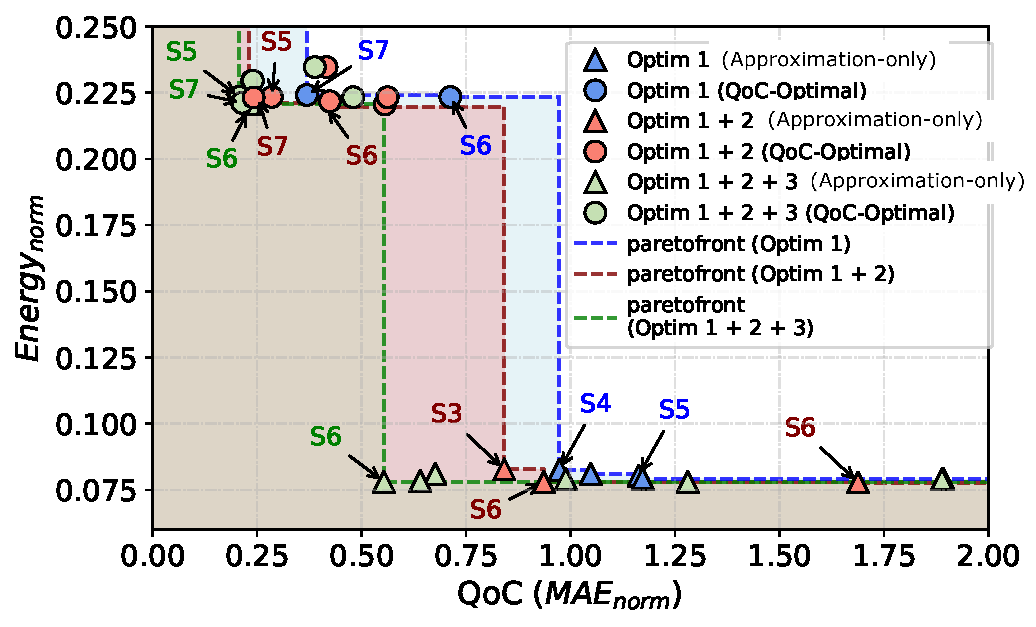
\includegraphics[width= 0.86\textwidth]{figs/lqg1_2.pdf}
    \caption{{\Gls{qoc}-Energy trade-offs for Optim 3. Pareto-front improvements over Optim 1 and Optim 2 are shown. Note that the energy here is a measure of the degree of approximation in the approximation-only mode. The lower the energy, the higher the degree of approximation. The reader is referred to \cite{de2020access} for more details on the energy-aware optimisation.}}
    \label{fig:optim3}
    %\vspace{-5 pt}
\end{figure}
We use the optimal \gls{lqg} control design~\cite{franklin1998digital} technique to design the approximation-aware controller for the system defined as follows:
\begin{align}
     \dot x(t) &= \Acont x(t) + \Bcont u(t), \nonumber \\
     y(t) &= \Ccont x(t) + e_i,
     \nonumber
\end{align}
where $e_i$ models the error due to approximation as measurement noise for the output.

\par Fig.\ \ref{fig:optim3} shows the \gls{qoc}-Energy trade-offs for Optim 3, approximation-aware \gls{lqg} control, for the \gls{lkas} case study. Recall from Section \ref{sec:ch6_lqr} that the results so far were obtained by using an \gls{lqr} controller. The control error of the \gls{lqr} controllers for the various pipeline settings was quantified as explained above and used to design an \gls{lqg} controller for each setting. We observe that the area under the Pareto curve for Optim 3 improves by 22\% and 15\% over Optim 1 and 2, respectively. This means that better trade-offs in terms of \gls{qoc} and energy are obtained by the \gls{lqg} controllers. It is important to mention that Optim 3 has \gls{qoc} improvements over Optim 2 but no energy improvements, as it does not influence the compute-intensive sensing stage (\taskS). This explains why the Pareto front only moves towards the left. Finally, the improvements from Optim 3 in approximation-only mode are higher than in \gls{qoc}-optimal mode. This is because, in approximation-only mode, faster sampling is not considered. So, control decisions at each actuation are valid longer. So, better decisions taken by the \gls{lqg} controller are more profound in approximation-only mode compared to \gls{qoc}-optimal mode.